\newcommand{\combineDivisions}{Hinweis: Wenn weniger als 5 Teams in einer der
Altersgruppen angemeldet sind, hat die Veranstaltungsleitung die Möglichkeit,
Altersgruppen zusammenzulegen. }

\newcommand{\declareExhibition}{Wenn insgesamt weniger als 5 Teams angemeldet
sind kann die Veranstaltung zur Ausstellung erklärt werden. }

\newcommand{\robotRequirements}{Autonomer Roboter, basierend auf einer
beliebigen Plattform, der \euro{1.500} oder weniger kostet und die folgenden
Designbedingungen erfüllt, die beim Check-In überprüft werden:}


\newcommand{\tournamentScoring}{
\begin{figure}[H]
	\centering
	\def\svgwidth{\columnwidth}
	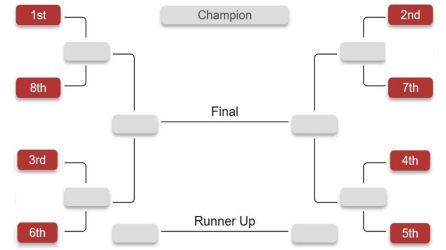
\includegraphics{tournament_score/tournament_score.pdf}
\end{figure}
}

\newcommand{\tournamentQualification}{Die aufsteigenden Teams werden
entsprechend ihrer Gesamtpunktzahl in den Turnierplan eingetragen (unten findet
ihr ein Beispiel für ein typisches Turnier mit 8 Teams). }

\newcommand{\combinedTournament}{
Hinweis: Wenn weniger als 8 Teams in allen Altersgruppen angemeldet sind, hat
die Veranstaltungsleitung die Möglichkeit, den Turnierplan entsprechend
anzupassen.
}

\newcommand{\scoreRuns}{
Die Veranstaltungsleitung legt die Anzahl der erlaubten offiziellen Läufe fest
und die Anzahl derjenigen offiziellen Läufe, die in die Gesamtwertung eingehen
auf deren Grundlage die besten 8 Teams ermittelt werden, welche am Turnier
teilnehmen.}

\newcommand{\lightConditions}{
Die Challenge kann in Bereichen mit natürlichen Licht stattfinden, welches die
Lichtverhältnisse auf dem Spielplan verändern kann. Teams sollten darauf
vorbereitet sein, diese natürlichen Bedingungen zu meistern. }
